%                                                                 aa.dem
% AA vers. 8.2, LaTeX class for Astronomy & Astrophysics
% demonstration file
%                                                       (c) EDP Sciences
%-----------------------------------------------------------------------
%
%\documentclass[referee]{aa} % for a referee version
%\documentclass[onecolumn]{aa} % for a paper on 1 column  
%\documentclass[longauth]{aa} % for the long lists of affiliations 
%\documentclass[rnote]{aa} % for the research notes
%\documentclass[letter]{aa} % for the letters 
%\documentclass[bibyear]{aa} % if the references are not structured 
% according to the author-year natbib style

%
\documentclass{aa}  

%
\usepackage{graphicx}
%%%%%%%%%%%%%%%%%%%%%%%%%%%%%%%%%%%%%%%%
\usepackage{txfonts}
%%%%%%%%%%%%%%%%%%%%%%%%%%%%%%%%%%%%%%%%
\usepackage{hyperref}
% To add links in your PDF file, use the package "hyperref"
% with options according to your LaTeX or PDFLaTeX drivers.
%
%\usepackage{url}
%\usepackage{fontawesome}

%\usepackage{xspace}
%\usepackage{subcaption}

\def\detJ{\mathrm{det}J}

\def\tein{\theta_{\mathrm{Ein}}}
\def\trad{\theta_{\mathrm{rad}}}
\def\tsis{\theta_{\mathrm{Ein}}^{\mathrm{(SIS)}}}
\def\meantsis{<\tsis>}
\def\stdtsis{\sigma(\tsis)}

\def\teinein{\theta_{\mathrm{Ein}}^*}
\def\betaein{\beta^*}

\def\toneobs{\theta_1^{\mathrm{obs}}}
\def\ttwoobs{\theta_2^{\mathrm{obs}}}

\def\moneobs{m_1^{\mathrm{obs}}}
\def\mtwoobs{m_2^{\mathrm{obs}}}

\def\asymm{\xi_{\mathrm{asymm}}}
\def\rmur{r_{\mu_r}}
\def\rmurobs{r_{\mu_r}^{(\mathrm{obs})}}
\def\mumin{\mu_{\mathrm{min}}}
\def\betamax{\beta_{\mathrm{max}}}
\def\betasl{\beta_{\mathrm{SL}}}

\def\hyperpars{\boldsymbol{\eta}}
\def\indpar{\boldsymbol{\psi}}
\def\indpari{\boldsymbol{\psi}_i}

\def\nsource{N_{\mathrm{s}}}
\def\nbkg{n_{\mathrm{bkg}}}

\def\psilens{\boldsymbol{\psi}_\mathrm{g}}
\def\psisource{\boldsymbol{\psi}_\mathrm{s}}
\def\psisourcetwo{\boldsymbol{\psi}_{\mathrm{s},2}}
\def\psisourcens{\boldsymbol{\psi}_{\mathrm{s},\nsource}}
\def\psisourcenobeta{\boldsymbol{\psi}_\mathrm{s}^{(-\boldsymbol\beta)}}

\def\Nlens{N_{\mathrm{lens}}}
\def\Nnot{N_{\mathrm{not}}}

\def\prlens{{\rm P}_\mathrm{g}}
\def\prsource{{\rm P}_\mathrm{s}}
\def\prlensone{{\rm P}_{\mathrm{g},1}}
\def\prlenstwo{{\rm P}_{\mathrm{g},2}}
\def\prsourceone{{\rm P}_{\mathrm{s},1}}
\def\prsourcetwo{{\rm P}_{\mathrm{s},2}}
\def\prsl{{\rm P}_\mathrm{{SL}}}
\def\prslone{{\rm P}_{\mathrm{SL},1}}
\def\prsltwo{{\rm P}_{\mathrm{SL},2}}

\def\prsourcenobeta{{\rm P}_\mathrm{s}^{(-\boldsymbol\beta)}}

\def\pdet{{\rm P}_\mathrm{det}}
\def\pdetone{{\rm P}_{\mathrm{det},1}}
\def\pdettwo{{\rm P}_{\mathrm{det},2}}
\def\crosssect{\sigma_\mathrm{{SL}}}

\def\data{\mathbf{d}}
\def\datai{\mathbf{d}_i}

\def\dlens{\mathbf{d}_{\mathrm{g}}}
\def\dsource{\mathbf{d}_{\mathrm{s}}}

\def\mlim{m_{\mathrm{max}}}

\def\Sref#1{Section~\ref{#1}\xspace}
\def\Fref#1{Figure~\ref{#1}\xspace}
\def\Tref#1{Table~\ref{#1}\xspace}
\def\Eref#1{Equation~\ref{#1}\xspace}

\newcommand{\ale}[1]{\textcolor{red}{\textbf{[Ale: #1]}}}

\def\pr{{\rm P}}

\defcitealias{S+C21}{Paper~I}
\defcitealias{Son21}{Paper~II}
\defcitealias{Son22}{Paper~III}
\setcitestyle{notesep={}}

\begin{document} 


   \title{Strong lensing selection effects}
   \titlerunning{Strong lensing selection effects}
   \authorrunning{Sonnenfeld et al.}

   \author{Alessandro Sonnenfeld\inst{1}
          }

   \institute{Leiden Observatory, Leiden University, Niels Bohrweg 2, 2333 CA Leiden, the Netherlands\\
              \email{sonnenfeld@strw.leidenuniv.nl}
             }

   \date{}

% \abstract{}{}{}{}{} 
% 5 {} token are mandatory
 
  \abstract
  % context heading (optional)
  % {} leave it empty if necessary  
    {
There are selection effects. They are important.
}
  % aims heading (mandatory)
   {
How important?
} 
   % methods heading (mandatory)
   {
I simulate lenses.
}
% results heading (mandatory)
   {
Results.
}
  % conclusions heading (optional), leave it empty if necessary 
   {
I conclude.
}
   \keywords{
             Gravitational lensing: strong --
             Galaxies: fundamental parameters
               }

   \maketitle
%
%________________________________________________________________

\section{Introduction}\label{sect:intro}

\citep{Son22} showed how to correct for selection effects in a population study of a sample of strong lenses. However, the practical realization of the \citep{Son22} method is challenging, as it requires 1) characterising the background source population, 2) 

The structure of this work is the following.
In \Sref{sect:indlenses} we study individual lens systems, to look for trends in the lensing cross-section with various lens and source properties.
In \Sref{sect:lenspop} we study 

I discuss the results in \Sref{sect:discuss} and draw conclusions in \Sref{sect:concl}.

The Python code used for the simulation and analysis of the lens sample can be found in a dedicated section of a GitHub repository\footnote{\url{https://github.com/astrosonnen/strong_lensing_tools}}.

%__________________________________________________________________

\section{Individual lenses}\label{sect:indlenses}

In this section we study how the probability of a strong lensing event varies as a function of 

\subsection{Axisymmetric lenses, point sources}

\begin{figure}
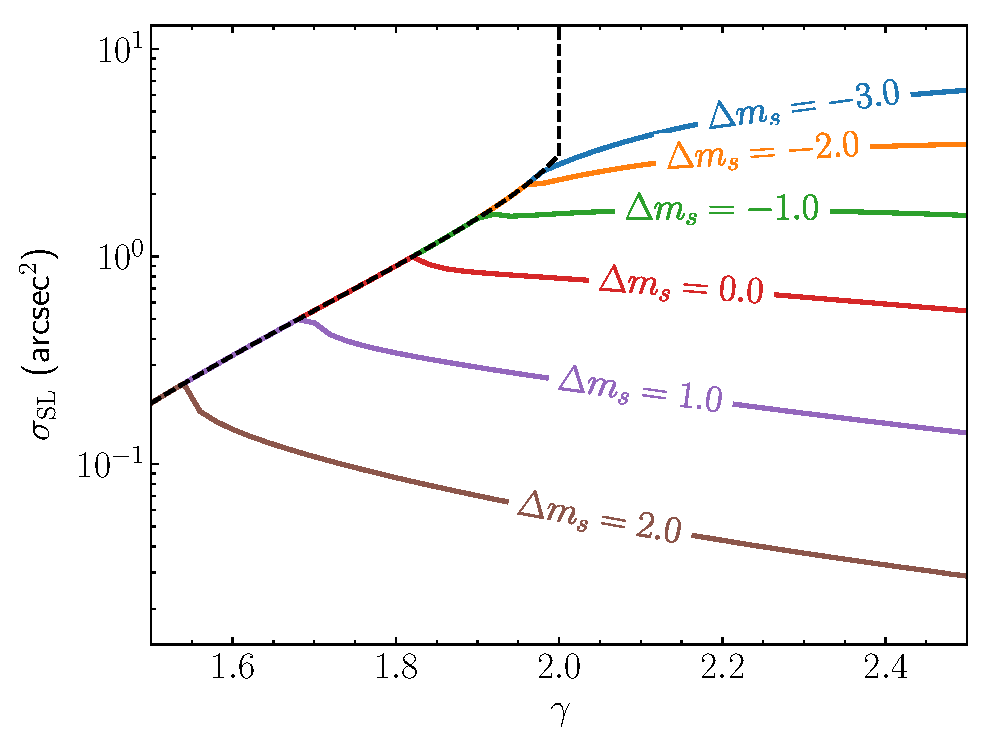
\includegraphics[width=\columnwidth]{axisymm_pl_crosssect.eps}
\caption{
Strong lensing cross-section of an axisymmetric power-law lens and a point source, as a function of the power-law slope $\gamma$.
The system is defined as a strong lens if at least two images are detected.
Different lines correspond to the difference $\Delta m$ between the source magnitude and the survey detection limit for a point source.
The dashed line marks the cross-section in the case in which at least two images are formed, regardless of their magnification.
}
\end{figure}

\subsection{Elliptical lenses, point sources}

\subsection{Elliptical lenses, extended sources}

%__________________________________________________________________

\section{Lens populations}\label{sect:lenspop}


%__________________________________________________________________

\section{Discussion and summary}\label{sect:discuss}

Discuss.

%\begin{acknowledgements}

%\end{acknowledgements}


\bibliographystyle{aa}
\bibliography{references}

\end{document}


